

% Chapter 1

\chapter{Robot} % Main chapter title

\label{Chapter2} % For referencing the chapter elsewhere, use \ref{Chapter1} 

\lhead{Capítulo 2. \emph{Robot}} % This is for the header on each page - perhaps a shortened title

%----------------------------------------------------------------------------------------

%--------------------------------------------------------
%Sección 1
%--------------------------------------------------------

\begin{figure}[htbp]
	\centering
		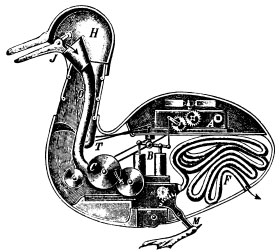
\includegraphics[width=0.6\textwidth]{./Figures/Duck_of_Vaucanson.jpg}
	%	\rule{35em}{0.5pt}
	%\caption[Robot Digesting Duck]{Digesting Duck, creado por Jacques de Vaucanson en 1739. Imagen tomada de Wikipedia.}
	\label{fig:Duck}
\end{figure}

Los robots ya son parte de la cultura pop, todos tienen al menos una idea de qué es un robot por la ciencia ficción o alguna noticia sobre los últimos avances. Incluso ya hay hogares en Chile que tienen una pequeña Robotina que recorre metódicamente todos los espacios de la casa para mantenerla sin polvo. A continuación un poco de historia y conceptos básicos de un robot.

\section{¿Qué es un robot?}

Un robot puede ser un software solamente o tener además una extensión física que le permita desempeñar tareas realizadas por el ser humano o que necesitan algo de inteligencia. El término robot se le atribuye al dramaturgo checo Karel Čapek, que en su obra R.U.R en 1921 (Rossum’s Universal Robots) utilizó la palabra \textit{robotnik} para referirse a ayudantes artificiales. Luego fue el escritor Isaac Asimov (1920-1992) quien,  gracias a su obra, difundió la palabra robótica haciendo referencia a la ciencia encargada de estudiar a los robots. Desarrolló las tres leyes de la robótica, que son una especie de normativa que regula el comportamiento de los robots en sus libros de Ciencia Ficción. Aparecidas por primera vez en el relato Runaround (1942), establecen lo siguiente:

\begin{enumerate}
\item Un robot no puede hacer daño a un ser humano o, por inacción, permitir que un ser humano sufra daño.
\item Un robot debe obedecer las órdenes dadas por los seres humanos, excepto si estas órdenes entrasen en conflicto con la 1ª Ley.
\item Un robot debe proteger su propia existencia en la medida en que esta protección no entre en conflicto con la 1ª o la 2ª Ley.
\end{enumerate}
La robótica como ciencia contempla el estudio de al menos seis áreas: La mecánica, la electrónica, la informática, el control automático, la física y la matemática.

Existen diferentes tipos y clases de robots, entre ellos con forma humana, de animales, de plantas. Todos se diferencian por sus capacidades y se clasifican en 4 formas:\begin{itemize}
\item Androides: robots con forma humana. Imitan el comportamiento de las personas, su utilidad en la actualidad es de solo experimentación. La principal limitante de este modelo es la implementación del equilibrio en el desplazamiento, pues es bípedo.
\item Móviles: se desplazan mediante una plataforma rodante (ruedas); estos robots aseguran el transporte de piezas de un punto a otro.
\item Zoomórficos: es un sistema de locomoción imitando a los animales. La aplicación de estos robots sirve, sobre todo, para el estudio de volcanes y exploración espacial.
\item Poliarticulados: mueven sus extremidades con pocos grados de libertad. Su principal utilidad es industrial, para desplazar elementos que requieren cuidados.
\end{itemize}

En ésta última se puede clasificar según su morfología en: Robots angulares o antropomórficos, robots cilíndricos, robots esféricos o polares, robots tipo SCARA, robots paralelos, robots cartesianos, entre otros. En este trabajo nos vamos a centrar solo en los robots Móviles con 2 ruedas.

En la historia hay varios intentos por construir estos ayudantes artificiales. A principios del siglo XVIII, Jacques de Vaucanson creó un autómata capaz de tocar la flauta, así como un pato mecánico que continuamente seguía su ciclo biológico.

En la actualidad las empresas KUKA, Honda y Sony, entre otras, construyen robots especialmente diseñados para la industria. Los robots que se utilizan en la industria, y los pocos que han llegado al hogar, son controlados por un algoritmo. Este es parte de un software que escribe una persona, donde se detalla la tarea que el robot debe realizar; tiene un modelo de los motores, partes y piezas para que así la máquina tenga información de como es, y pueda ejecutar la tarea para la cual se le programó. Si se interfiere con el entorno del robot, por ejemplo moviendo 1 [cm], fuera del rango de los sensores, el perno que debe apretar algún robot industrial que ensambla autos, este no podrá \textit{encontrarlo}. No todos los robots comerciales que existen hoy en día son capaces de adaptarse a cambios en el entorno (hay algunos que poseen sistemas de visión que permiten hacer estas correcciones), y menos ser capaces de generar una imagen de sí mismos que les permita entender qué sucede y recuperarse de fallas. Además de estos robots industriales hay algunos que son para uso militar que permiten desactivar bombas y rescatar personas. También existen robots que son capaces de asistir a una persona con discapacidades o incluso un robot acuático con una cámara que puede permitir a una persona recorrer el fondo del océano. 

\begin{figure}[htbp]
	\centering
		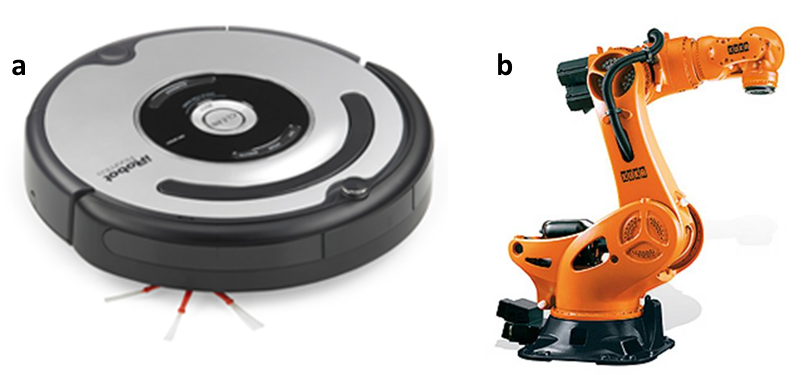
\includegraphics[width=\textwidth]{./Figures/RobotsInd.png}
		\rule{35em}{0.5pt}
	\caption[Robots Roomba y KUKA]{\textbf{a. }Robot Roomba, primer Robot doméstico vendido en Chile. Imagen tomada de \cite{Forlizzi:2006:SRD:1121241.1121286} \textbf{b.} Robot industrial KUKA KR 1000 TITAM. Imagen tomada de kuka-robotics.com}
	\label{fig:Roomba y KUKA}
\end{figure}

Para que un robot pueda hacer cosas es necesario programar el software de control. Se debe tener un modelo detallado de los motores y sensores que se poseen y es tarea del programador hacer la abstracción necesaria para poder darle sentido al movimiento del conjunto de motores. Cada motor aporta con un grado de libertad, o por su sigla en ingles DOF (degree of freedom), ver Figura \ref{fig:grados de libertad}. Los Grados de libertad hacen referencia al número de movimientos independientes que se pueden realizar. En otras palabras, un grado de libertad es la capacidad de moverse a lo largo de un eje (movimiento lineal) o de rotar en torno a un eje (movimiento rotacional). Por ejemplo, un auto posee 3 grados de libertad, dos de posición y uno de orientación. 

Si hablamos de un robot de 4 extremidades, con 3 grados de libertad en cada una, el programador debe ser capaz de indicar la secuencia de activación de cada motor. Primero debe hacer que el robot mueva una extremidad y luego con la suma de las 4 lograr desplazarse. Estamos hablando de 12 motores que pueden moverse de forma independiente, lo cual genera infinitas soluciones y no todas posibles debido a las restricciones físicas de la construcción misma del robot.

\begin{figure}[htbp]
	\centering
		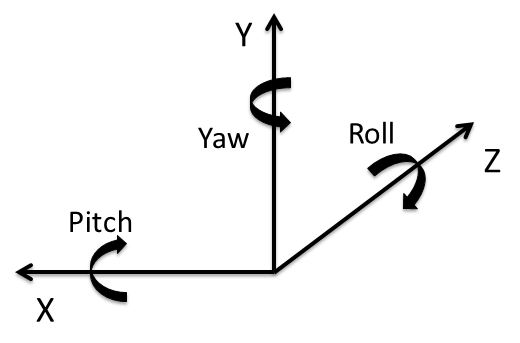
\includegraphics[width=\textwidth]{./Figures/6DOF.png}
		\rule{35em}{0.5pt}
	\caption[Grados de libertad]{Cada motor en un robot aporta un grado de liberdad. Acá hay seis grados de libertad, tres son de desplazamiento y tres son de orientación.}
	\label{fig:grados de libertad}
\end{figure}

Para programar el movimiento un robot cuadrúpedo es útil observar a la naturaleza, buscar animales que tengan una forma similar y tratar de replicar su movimiento. En ese sentido la naturaleza siempre ha sido una gran fuente de inspiración para las creaciones del ser humano. Actualmente el interés se ha volcado a investigar los enjambres de animales, que aunque están compuestos por muchos individuos de comportamiento simple son capaces de organizarse de alguna manera para cumplir con tareas más complejas. Entender y aplicar este tipo de comportamientos a grupos de robots puede ser de gran ayuda para cumplir con tareas distribuidas donde no sea suficiente el trabajo de un solo robot, si no más se requiera el trabajo de varios.


